% ============================================================
% 正文：Experimental Results
% 作者：Kehui Chen, Jacky Keung, Xiaoxue Ma
% 主题：MCP 故障定位（fault localization）根因实证研究
% ============================================================
\section{Experimental Results}\label{sec:results}

Interviewees have 1--20 years of working experience and work in teams of 6--160 members. They
are proficient in mainstream full-stack languages including Java, Python, C++, and Rust. All
enterprise names are anonymised for academic ethics and data privacy. We adopted open coding
to analyse the interview data and summarise results with practical cases.

\subsection{RQ1: Types of Runtime Faults in MCP Pipelines}

Our dataset is the \textbf{342 active real bugs} mined from the official
\verb|modelcontextprotocol/python-sdk| issue tracker, of which \textbf{49 are reproduced at
runtime} over the production Streamable HTTP transport (see Section~\ref{sec:setup}). Applying
the four-layer origin taxonomy (Fig.~\ref{fig:layer}), the 49 reproduced bugs span all four
layers: Host (4), Client (4), Server (36), and Transport (5). Each bug is bound to a real issue
number, so no fault is fabricated.

Crucially, the fault distribution reveals a stark asymmetry in \emph{how faults are
reported} (Fig.~\ref{fig:layer}). Of the 36 Server-origin bugs, the majority are correctly
reported within their own layer, but their real root cause / error value is often replaced by a
generic message (see RQ2). More strikingly, \emph{none} of the 13 non-Server bugs is reported
at its true origin: every Host-, Client-, and Transport-origin fault is surfaced in a way that
does not identify the layer where it actually originated. In other words, a developer reading
the raw output of a fault that genuinely starts in the Host, Client, or Transport layer has
\emph{no} reliable signal pointing back to that layer.

\noindent
\begin{minipage}{\linewidth}
  \centering
  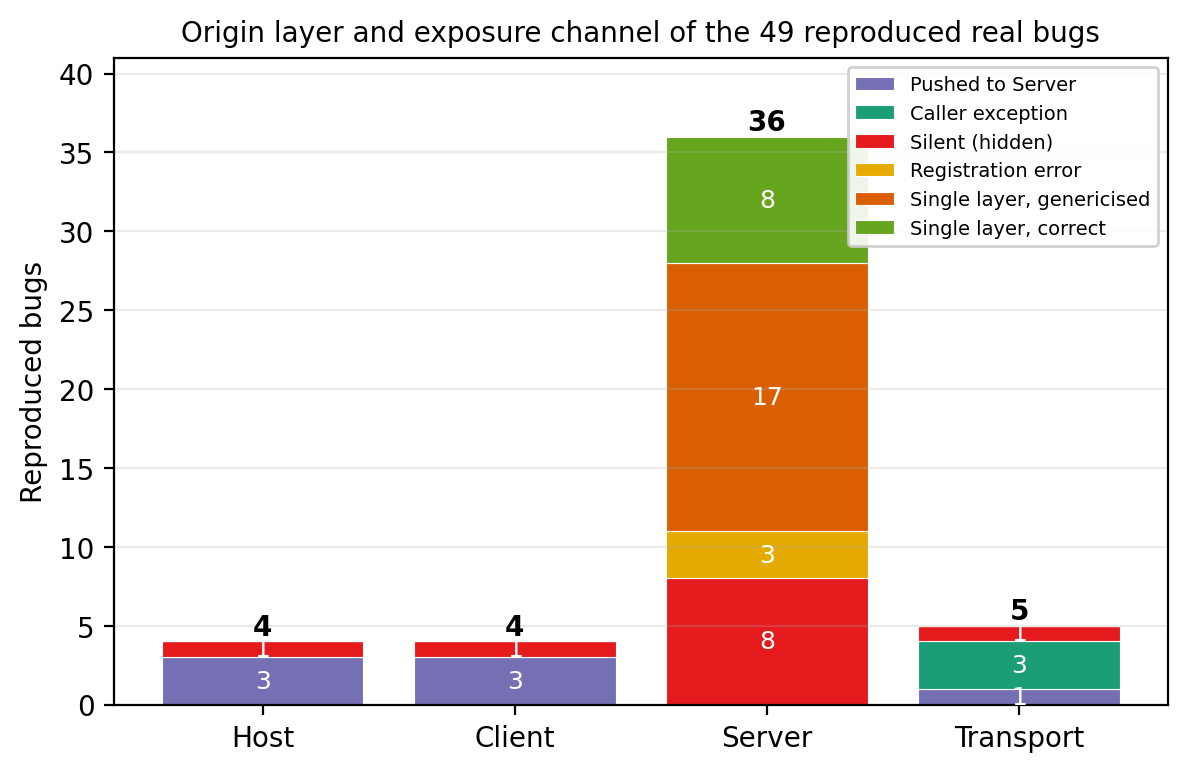
\includegraphics[width=\linewidth]{figs/fig_layer_distribution}
  \captionof{figure}{Fault distribution across the four-layer MCP fault taxonomy over the 49 reproduced real bugs.}
  \label{fig:layer}
\end{minipage}

\noindent
\begin{tabularx}{\linewidth}{@{}>{\centering\arraybackslash}m{2.2em}!{\vrule width 1pt}>{\arraybackslash}X@{}}
\makecell{\LARGE \faIcon[regular]{lightbulb}} &
\textbf{Finding 1.} MCP runtime faults are distributed across all four layers, yet the layer at which a fault is \emph{reported} hardly ever matches the layer at which it \emph{originated}. None of the 13 non-Server bugs is surfaced at its true origin, so the raw output gives a developer no reliable clue to the real root-cause layer.
\end{tabularx}

\subsection{RQ2: Manifestation-Root-Cause Mismatch}

Fig.~\ref{fig:alluvial} gives the full picture of the 49 reproduced bugs as a flow from their
\emph{origin layer} (left) to the \emph{exposure channel} through which the SDK actually
surfaces each fault (right), with one ribbon per bug (labelled by issue number). It makes the
core problem visually explicit: the layer a developer \emph{sees} (right) rarely matches the
layer where the fault really \emph{originated} (left).

\begin{figure*}[!t]
  \centering
  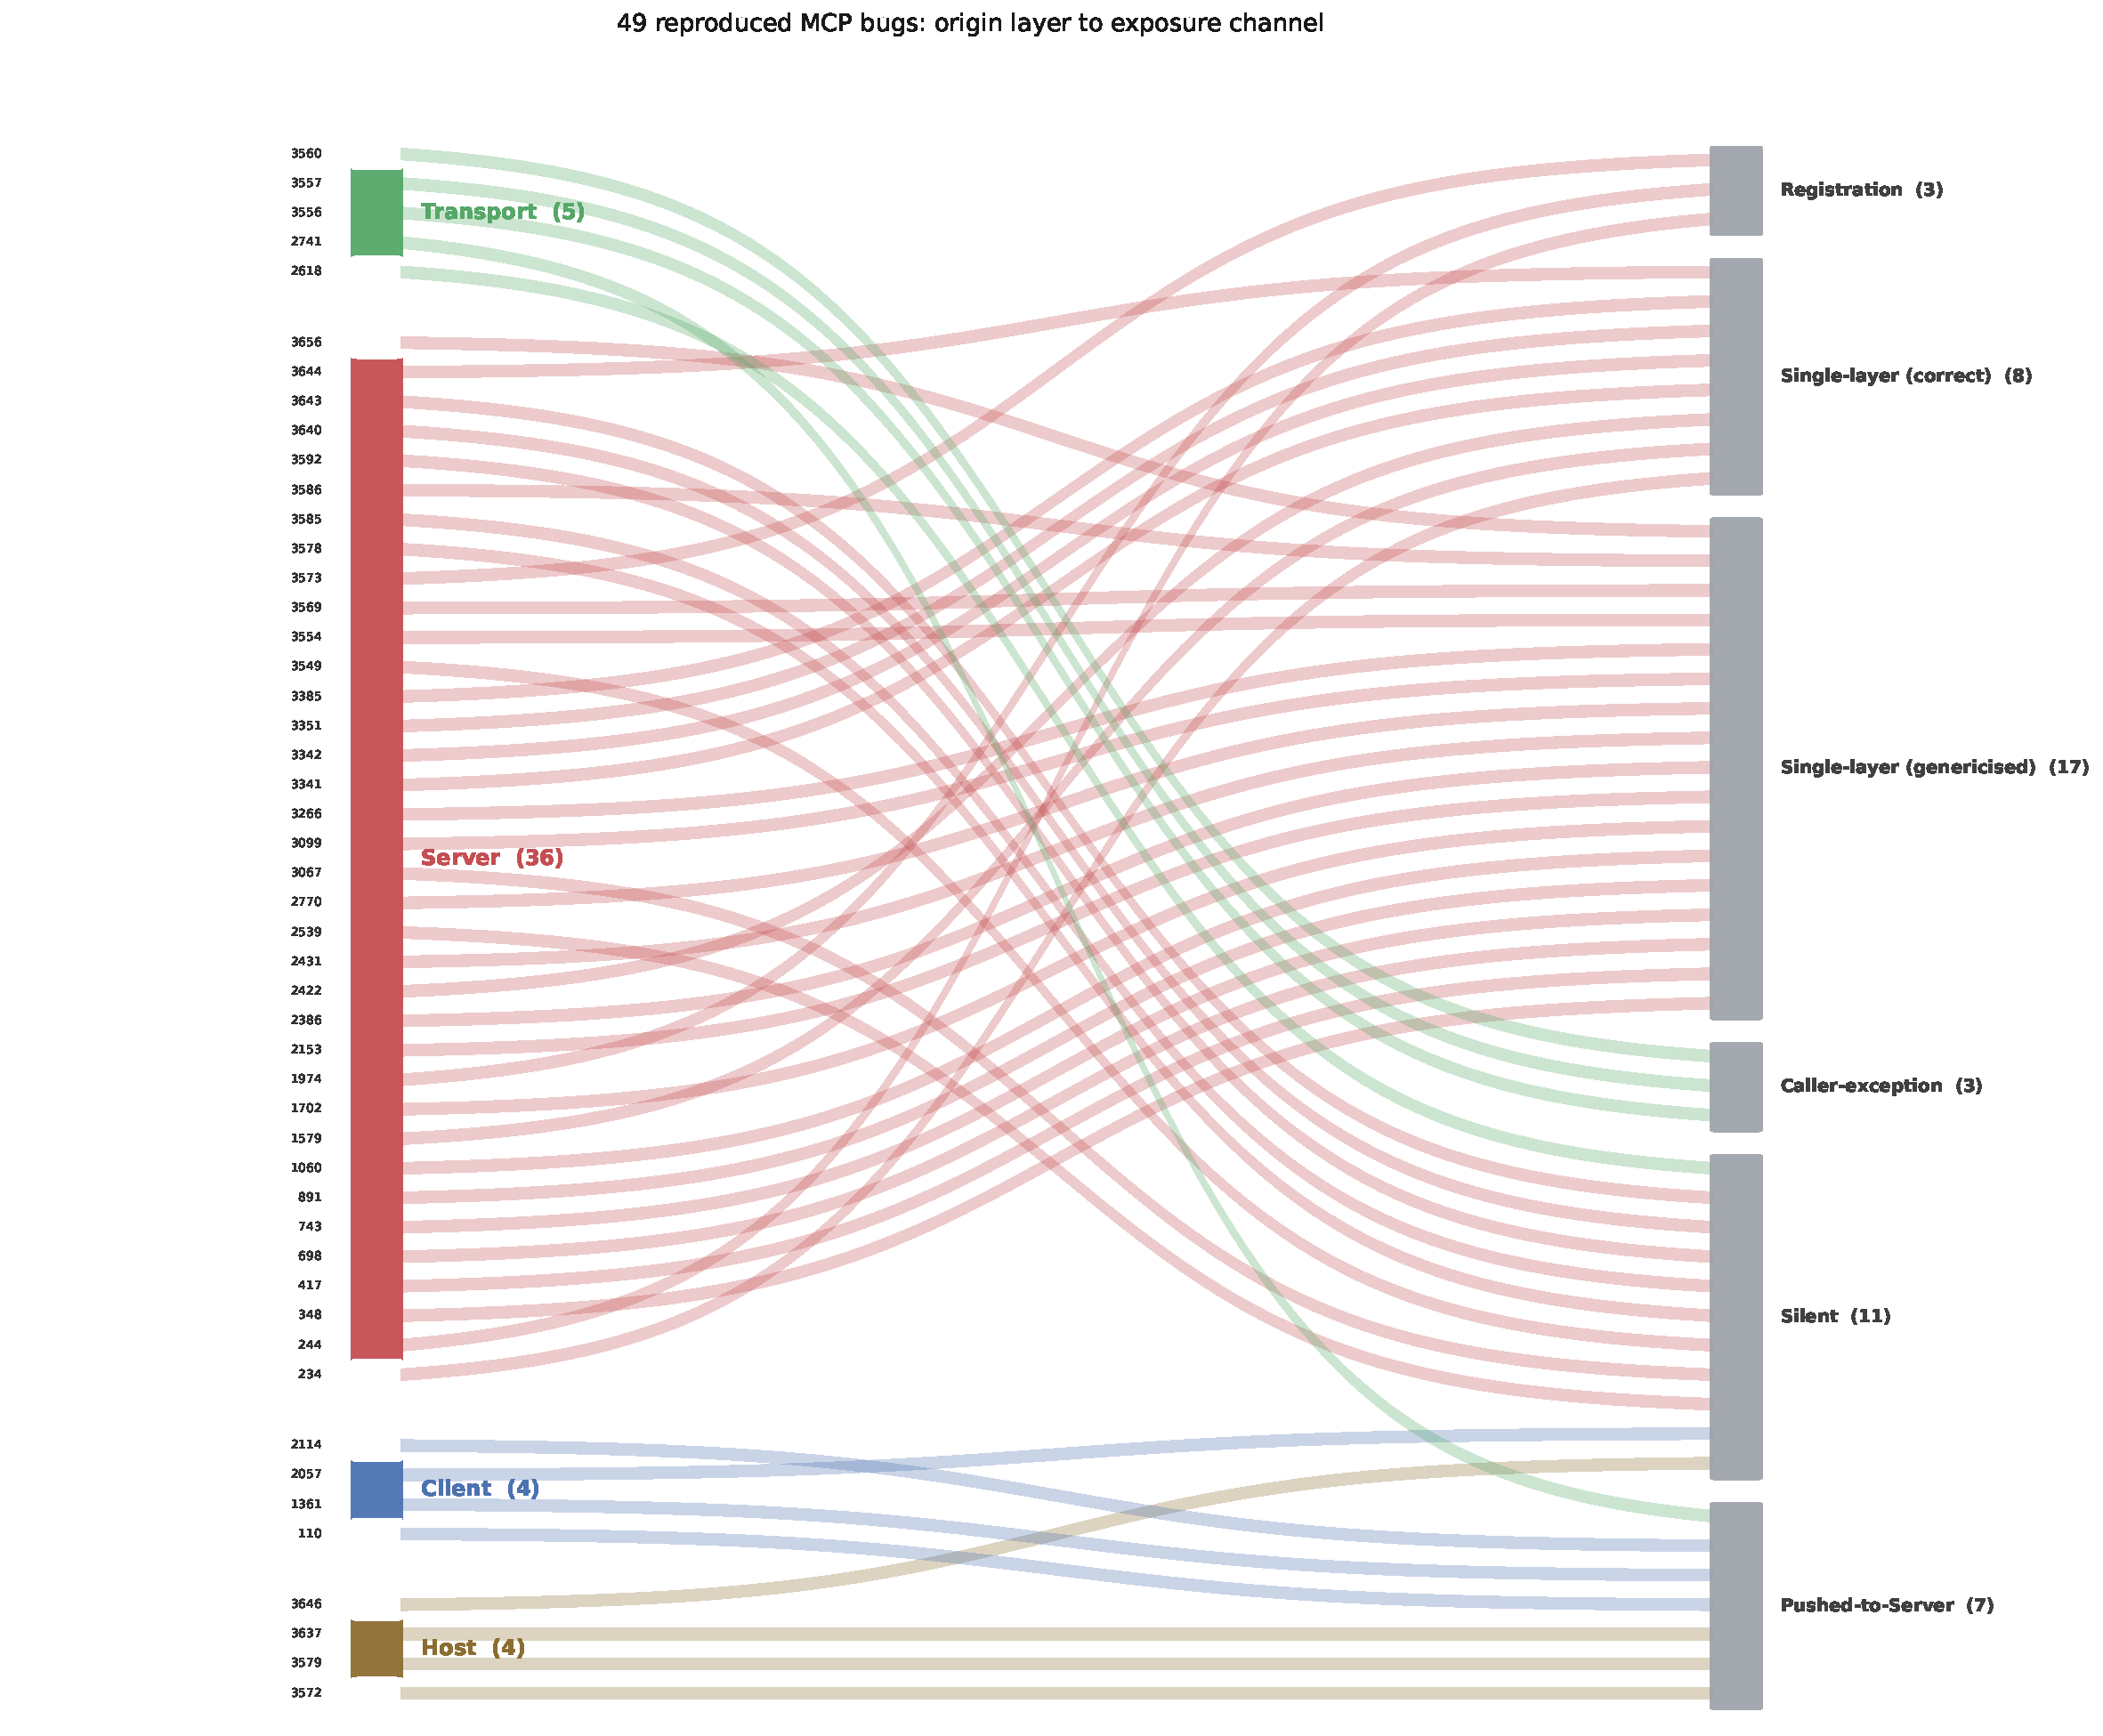
\includegraphics[width=0.92\textwidth]{figs/fig_main_alluvial_with_ids}
  \caption{Alluvial overview of the 49 reproduced real bugs from origin layer to exposure channel.}
  \label{fig:alluvial}
\end{figure*}

MCP SDKs surface errors at the layer where they are \emph{observed}, not necessarily where
they \emph{originated}. We quantify this with an observation-driven \emph{three-channel
exposure model}: for every one of the \textbf{13 non-Server bugs} among the 49 reproduced, we
inspect the raw SDK output and assign it to exactly one of the ways in which the fault is
exposed (or hidden). The result (Fig.~\ref{fig:alluvial}) shows that \emph{no} non-Server bug is
correctly localised at its true origin; instead, each is exposed through one of the
non-informative channels:

\begin{itemize}
  \item \textbf{Pushed to the Server layer (7/13):} an upstream Host or Client fault is
        re-surfaced by the Server-side tool-execution pipeline as \texttt{Error executing tool
        X ...} with \texttt{is\_error=True}, so the error \emph{looks} like a Server bug.
  \item \textbf{Caller-side raw exception (3/13):} a Transport fault (e.g.\ calling a tool
        after session closure, or a cancelled request) is thrown directly in the calling code
        as a bare Python exception, rather than being reported by the tool-related layer.
  \item \textbf{Silent (3/13):} the fault is accepted and a successful
        (\texttt{is\_error=False}) status is returned, so it is invisible to any error-based
        monitor.
\end{itemize}

Excluding the silent channel (which we treat separately in RQ3), \textbf{10/13 = 76.9\%}
non-Server bugs are \emph{manifestation-root-cause mismatched}: the reported layer differs
from the true origin (7 pushed to Server + 3 caller-side exceptions). Moreover, considering
all three channels together, \textbf{all 13/13 non-Server bugs are not correctly localised at
their true origin}. A further, independent mechanism degrades even the Server-origin reports:
\textbf{17/49 = 34.7\%} of the reproduced bugs are \emph{genericised} --- although reported at
the correct (Server) layer, the SDK replaces the real root cause / error value with the generic
\texttt{Error executing tool X} string, so the specific cause (a \texttt{TypeError}, a
non-pickle-safe \texttt{McpError}, a CWE-209-sensitive value) is stripped away. The complete
per-bug breakdown is given in Table~\ref{tab:repro49}.

A representative example of the ``pushed to Server'' channel is bug \#3572: the Host sends a
tool argument of the wrong type, so the actual defect originates in the Host-side caller.
However, the validation error is thrown and reported by the Server-side tool execution pipeline,
i.e.\ as \texttt{Error executing tool lookup: 1 validation error...}. A developer reading the
error log is therefore misled to suspect a bug inside the Server tool logic, when the real fault
lies in an upstream caller component.

\noindent
\begin{tabularx}{\linewidth}{@{}>{\centering\arraybackslash}m{2.2em}!{\vrule width 1pt}>{\arraybackslash}X@{}}
\makecell{\LARGE \faIcon[regular]{lightbulb}} &
\textbf{Finding 2.} MCP SDK errors are exposed at the layer where they are \emph{observed}, not where they \emph{originated}. None of the 13 non-Server bugs is localised at its true origin: 7 are pushed to the Server layer, 3 surface as bare caller-side exceptions, and 3 are silent. This yields a 76.9\% generalised manifestation-root-cause mismatch (10/13); a further 17/49 = 34.7\% of (Server-origin) bugs are genericised, their real root cause replaced by \texttt{Error executing tool X}. These are principal technical causes of the reported difficulty in locating the true root cause.
\end{tabularx}

% ★【中文说明】新增：49 条真实复现 bug 的数据层表格（按暴露通道分组，含 issue 号/起源层/根因）。
%   替代旧合成 MCP-Fault-20(80 runs) 作为 RQ1/RQ2 的核心证据表。三通道/静默/错位只在此 49 条上算。
% ★[English] New: data-layer table of the 49 genuinely reproduced real bugs, grouped by exposure
%   channel, with issue number / origin layer / root cause. Supersedes the synthetic MCP-Fault-20
%   (80 runs) as the core evidence table for RQ1/RQ2. Channels computed only on these 49.
\begin{table*}[!t]
\centering
\caption{The 49 reproduced real bugs classified by origin layer and the channel through which the MCP SDK exposes each fault.}
\label{tab:repro49}
\scriptsize
\renewcommand{\arraystretch}{1.03}
\setlength{\tabcolsep}{1.25pt}
\begin{tabularx}{\textwidth}{@{}>{\centering\arraybackslash}X{0.7} >{\centering\arraybackslash}c >{\centering\arraybackslash}c >{\arraybackslash}X{1.3}@{}}
\toprule
\textbf{Channel} & \textbf{Issue} & \textbf{Origin} & \textbf{Exposure channel / root cause} \\
\midrule
\emph{Pushed-to-Server (7)} & \#110 & Client & Server returns non-UTF-8 bytes; client JSON decode error masked as \texttt{Error executing tool bad} \\
\emph{Pushed-to-Server (7)} & \#1361 & Client & \texttt{call\_tool} exception swallowed, re-surfaced as \texttt{Error executing tool boom} \\
\emph{Pushed-to-Server (7)} & \#2114 & Client & \texttt{ExceptionGroup} obscures the real tool error, masked as \texttt{Error executing tool boom} \\
\emph{Pushed-to-Server (7)} & \#2741 & Transport & in-session exception masked as \texttt{Error executing tool boom}; real cause in \texttt{Session crashed} log \\
\emph{Pushed-to-Server (7)} & \#3572 & Host & tool validation error echoes the rejected input; reported as \texttt{Error executing tool lookup} \\
\emph{Pushed-to-Server (7)} & \#3579 & Host & unknown tool requested from a component-less server; reported at Server \\
\emph{Pushed-to-Server (7)} & \#3637 & Host & Pydantic model param not flattened; flat client arg dict rejected at Server \\
\midrule
\emph{Silent (11)} & \#2057 & Client & \texttt{id:null} misclassified as notification, accepted (HTTP 202), never rejected \\
\emph{Silent (11)} & \#2539 & Server & optional \texttt{None} field serialised as JSON \texttt{null}; wrong result shape returned \\
\emph{Silent (11)} & \#2618 & Transport & \texttt{MCP-Protocol-Version} header vs body mismatch not validated (HTTP 200) \\
\emph{Silent (11)} & \#3067 & Server & misspelled argument silently dropped (\texttt{extra=ignore}); returns plausible result \\
\emph{Silent (11)} & \#3549 & Server & 20 concurrent calls lose updates (result=1, expected 20); no error flag \\
\emph{Silent (11)} & \#3578 & Server & duplicate tool registration silently keeps the first version \\
\emph{Silent (11)} & \#3585 & Server & unregistered MIME type (\texttt{image/jpg}) emitted without error \\
\emph{Silent (11)} & \#3592 & Server & stale-cache fallback marker returned as success (\texttt{is\_error} mismatch) \\
\emph{Silent (11)} & \#3640 & Server & unknown \texttt{ServerCapabilities} keys silently dropped from advertised capabilities \\
\emph{Silent (11)} & \#3643 & Server & \texttt{UserList} prompt result rendered as one stringified message \\
\emph{Silent (11)} & \#3646 & Host & unknown extra tool argument silently accepted (no opt-in rejection) \\
\midrule
\emph{Caller-exception (3)} & \#3556 & Transport & client treats 404 (dead session) as terminal; raises \texttt{ExceptionGroup} \\
\emph{Caller-exception (3)} & \#3557 & Transport & malformed body answered with \texttt{-32602} (should be \texttt{-32600}); HTTP 400 \\
\emph{Caller-exception (3)} & \#3560 & Transport & no default timeout; slow tool blocks caller, raises \texttt{ExceptionGroup} \\
\midrule
\emph{Single-layer genericised (17)} & \#348 & Server & no way to set \texttt{isError=True} for arbitrary tool result; real error masked \\
\emph{Single-layer genericised (17)} & \#417 & Server & internal error masked as \texttt{Error executing tool boom} \\
\emph{Single-layer genericised (17)} & \#698 & Server & tool exception value not revealed; masked as \texttt{Error executing tool boom} \\
\emph{Single-layer genericised (17)} & \#743 & Server & root cause not logged; masked as \texttt{Error executing tool boom} \\
\emph{Single-layer genericised (17)} & \#891 & Server & \texttt{dict+str} real \texttt{TypeError} masked as \texttt{Error executing tool f} \\
\emph{Single-layer genericised (17)} & \#1060 & Server & \texttt{PydanticSchemaGenerationError} for Image masked as \texttt{Error executing tool img} \\
\emph{Single-layer genericised (17)} & \#1702 & Server & tool output fails outputSchema validation; masked as \texttt{Error executing tool get\_name} \\
\emph{Single-layer genericised (17)} & \#2153 & Server & handler should raise; masked as \texttt{Error executing tool boom} \\
\emph{Single-layer genericised (17)} & \#2386 & Server & CWE-209 sensitive value (\texttt{password=abc}) sanitised; real ValueError masked \\
\emph{Single-layer genericised (17)} & \#2431 & Server & \texttt{McpError} not pickle-safe; masked as \texttt{Error executing tool boom} \\
\emph{Single-layer genericised (17)} & \#2770 & Server & \texttt{McpError} swallowed as \texttt{isError:true}; masked \\
\emph{Single-layer genericised (17)} & \#3099 & Server & field alias in schema but invalid Python keyword; masked as \texttt{Error executing tool ext} \\
\emph{Single-layer genericised (17)} & \#3266 & Server & tool-call exception not logged; masked as \texttt{Error executing tool boom} \\
\emph{Single-layer genericised (17)} & \#3554 & Server & non-UTF-8 bytes output crashes; masked as \texttt{Error executing tool get\_bytes} \\
\emph{Single-layer genericised (17)} & \#3569 & Server & non-ToolError surfaced; masked as \texttt{Error executing tool fragile2} \\
\emph{Single-layer genericised (17)} & \#3586 & Server & non-ToolError surfaced; masked as \texttt{Error executing tool fragile} \\
\emph{Single-layer genericised (17)} & \#3656 & Server & \texttt{Audio(data=b"")} raises while \texttt{Image} works; masked as \texttt{Error executing tool a} \\
\midrule
\emph{Single-layer correct (8)} & \#234 & Server & unknown tool returns \texttt{is\_error=True} (wrong \texttt{is\_error} semantics) \\
\emph{Single-layer correct (8)} & \#1579 & Server & \texttt{read\_resource} returns wrong error code on not-found \\
\emph{Single-layer correct (8)} & \#2422 & Server & \texttt{ToolNotFoundError} vs generic \texttt{ToolError} (wrong error granularity) \\
\emph{Single-layer correct (8)} & \#3341 & Server & non-finite float (\texttt{nan}) fails structured-content validation \\
\emph{Single-layer correct (8)} & \#3342 & Server & prompt validation error collapsed to \texttt{Internal server error} \\
\emph{Single-layer correct (8)} & \#3351 & Server & input-validation discards jsonschema field detail \\
\emph{Single-layer correct (8)} & \#3385 & Server & non-finite float (\texttt{inf}) produces invalid JSON in text content \\
\emph{Single-layer correct (8)} & \#3644 & Server & outputSchema in validation mode but content serialised by alias (schema mismatch) \\
\midrule
\emph{Registration-time (3)} & \#244 & Server & \texttt{@app.resource()} rejects \texttt{ctx: Context}; \texttt{ValueError} at registration \\
\emph{Registration-time (3)} & \#1974 & Server & \texttt{find\_context\_parameter} fails on callable class; \texttt{AttributeError} at registration \\
\emph{Registration-time (3)} & \#3573 & Server & \texttt{-> Iterator} annotation raises \texttt{PydanticSchemaGenerationError} at registration \\
\bottomrule
\end{tabularx}
\vspace{0.35em}
\parbox{\textwidth}{\scriptsize\raggedright
\textit{Note:} ``Issue'' is the GitHub issue number of \texttt{modelcontextprotocol/python-sdk}.
``Origin'' is the layer where the root cause lies. The ``Channel'' describes how the SDK \emph{exposes}
the fault: \emph{Pushed-to-Server} (a non-Server fault reported at the Server layer); \emph{Silent}
(\texttt{is\_error=False}, the logical error hidden); \emph{Caller-exception} (a raw Python / HTTP
exception in the calling code); \emph{Single-layer genericised} (Server-origin, but the real root
cause replaced by \texttt{Error executing tool X}); \emph{Single-layer correct} (Server-origin,
correctly reported with detail retained); \emph{Registration-time} (the server cannot build /
register a tool). The 17 ``genericised'' Server-origin bugs are reported at the correct layer but
their real root cause / error value is replaced by the generic \texttt{Error executing tool X} string.}
\end{table*}

\subsection{RQ3: Silent Failures}

Some erroneous inputs do not trigger any error flag at all. Among the 49 reproduced real bugs,
\textbf{11 (22.4\%)} exhibit silent failure: the SDK returns an outward-looking successful
status with \texttt{is\_error=False}, despite an underlying logical input or execution error.
These span all four layers and are not an artefact of a single category of defect.

Fig.~\ref{fig:silent} shows the distribution of these silent bugs by origin layer; several of
the most \textit{damaging} real-world defects are silent, including:
\begin{itemize}
  \item \textbf{\#3549 (concurrent lost update):} 20 concurrent calls to a counter return
        \texttt{1} instead of \texttt{20}, with \texttt{is\_error=False} --- the race is
        completely invisible to any error-based monitor.
  \item \textbf{\#3578 (duplicate tool registration):} registering a tool twice produces only a
        WARNING (\texttt{Tool already exists}) and silently keeps the first version.
  \item \textbf{\#3067 (misspelled argument):} a typo in a tool-call argument is silently
        dropped (\texttt{extra=ignore}) and a plausible result is returned.
  \item \textbf{\#2057 (null id):} a JSON-RPC request with \texttt{id:null} is misclassified as
        a notification and accepted (HTTP 202), never rejected.
\end{itemize}

\noindent
\begin{minipage}{\linewidth}
  \centering
  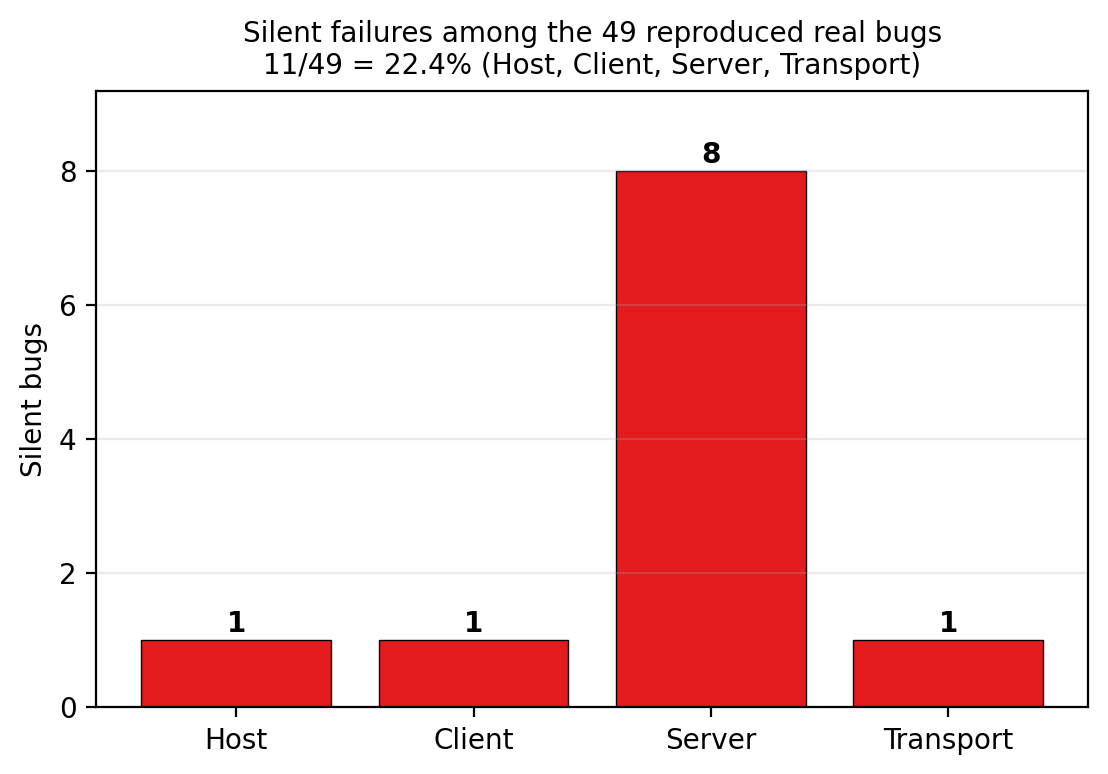
\includegraphics[width=\linewidth]{figs/fig_silent_failure}
  \captionof{figure}{Silent failures account for 22.4\% (11/49) of the reproduced real bugs.}
  \label{fig:silent}
\end{minipage}

\noindent
\begin{tabularx}{\linewidth}{@{}>{\centering\arraybackslash}m{2.2em}!{\vrule width 1pt}>{\arraybackslash}X@{}}
\makecell{\LARGE \faIcon[regular]{lightbulb}} &
\textbf{Finding 3.} Silent failures occur in 11/49 = 22.4\% of the reproduced real bugs, and include several of the most damaging defects --- a concurrent lost update (\#3549), a duplicate tool registration (\#3578), a silently-dropped misspelled argument (\#3067) and a null-id request accepted as a notification (\#2057). These defects are invisible to ordinary monitoring pipelines.
\end{tabularx}

\subsection{RQ4: Why Fault Localisation Is Hard, and How to Fix It}

\subsubsection{Demand-side evidence}

The interviews reveal fault localisation as the leading operational obstacle. In our open
coding, fault localisation emerged as the most frequently raised and most emphatically
emphasised theme: all 20 practitioners (20/20) named quickly locating the problem on a
malfunction as a top troubleshooting obstacle, and 16 participants (16/20) explicitly pointed
out the lack of standardised MCP diagnostic tools. Currently, fault tracing relies heavily on
manual work, accompanied by incomplete and unstructured logs, which greatly reduces
troubleshooting efficiency. Practitioners therefore strongly expect dedicated automated tools
to locate bugs, analyse logs, and identify root causes during routine operation and
maintenance. Because these are qualitative self-reports, we stress that this remains
\emph{demand-side} evidence; we verify it objectively in the next subsection.

\noindent
\begin{tabularx}{\linewidth}{@{}>{\centering\arraybackslash}m{2.2em}!{\vrule width 1pt}>{\arraybackslash}X@{}}
\makecell{\LARGE \faIcon[regular]{lightbulb}} &
\textbf{Finding 4.} Practitioners report that fault localisation is the single biggest obstacle in MCP deployment, and that manual log-based tracing, with incomplete and unstructured logs, is the dominant cause. They expect automated, standardised tools.
\end{tabularx}

\subsubsection{Objective verification of the demand with a surface-text LLM agent}

To verify this subjectively reported pain point objectively, we ran a surface-text
diagnostic agent over the \textbf{49 genuinely reproduced real bugs}. The agent is a large
language model (DeepSeek through the CityU proxy, temperature 0) that reads only the raw error
or success text returned by the MCP SDK for each bug and predicts the layer at which the fault
\emph{originated} (Host, Client, Server, or Transport). Crucially, we strip any ground-truth
layer metadata so that the model cannot exploit a shortcut: the agent sees exactly the message a
monitoring tool or human developer would see.

As shown in Fig.~\ref{fig:diag} (baseline), the agent achieves an overall
root-cause localisation accuracy of \textbf{77.6\%} (38/49). The failure is systematic rather
than random: it correctly localises \textbf{100\%} (36/36) of Server-origin bugs and 40\% (2/5)
of Transport-origin bugs, but \emph{0\%} of Host- and Client-origin faults. Because the overall
figure is inflated by the 36 Server-origin bugs (reported and localised correctly at the Server
layer), we report the \textbf{13 non-Server-origin bugs} as the honest hard-case number: the
agent localises only \textbf{15.4\%} (2/13) of them. In other words, when the true root cause
lies outside the Server layer, a surface-text diagnostic agent is \emph{almost always} misled
into blaming the Server. This is precisely the confusion the interviewed practitioners describe.

As a negative control, we also run the same agent with a \emph{leaky} hint that names the
exposure channel verbatim (e.g.\ ``pushed-to-Server'' / ``silent''). This does
not help: the leaky control is \emph{lower} on the non-Server bugs (0.0\%, vs.\ 15.4\% baseline),
confirming that the honest 77.6\%/15.4\% figure is \emph{not} relying on any shortcut --- and,
more importantly, that the raw SDK error text genuinely carries too little signal to localise
non-Server faults.

Because committing to a single verdict may be too harsh, we also ask the agent to \emph{rank} all
four layers and measure how many guesses it needs to localise the bug, i.e.\ to reach the layer
where the fault truly originated (Table~\ref{tab:topk}). Over all 49 bugs the agent localises the
correct layer on its \textbf{1st guess} 79.6\% of the time, on its 2nd 87.8\%, and on its 3rd
95.9\%. The hard cases
remain hard: on the 13 non-Server bugs the agent is correct on its 1st guess only
\textbf{23.1\%} of the time, on its 2nd 53.8\%, and on its 3rd \textbf{84.6\%} --- the two still
missed at the 3rd guess are silent bugs reported at a misleading layer. A developer would therefore still need up to three guesses to reliably reach a
non-Server root cause, confirming that surface text alone is insufficient for dependable
localisation.

\noindent
\begin{minipage}{\linewidth}
  \centering
  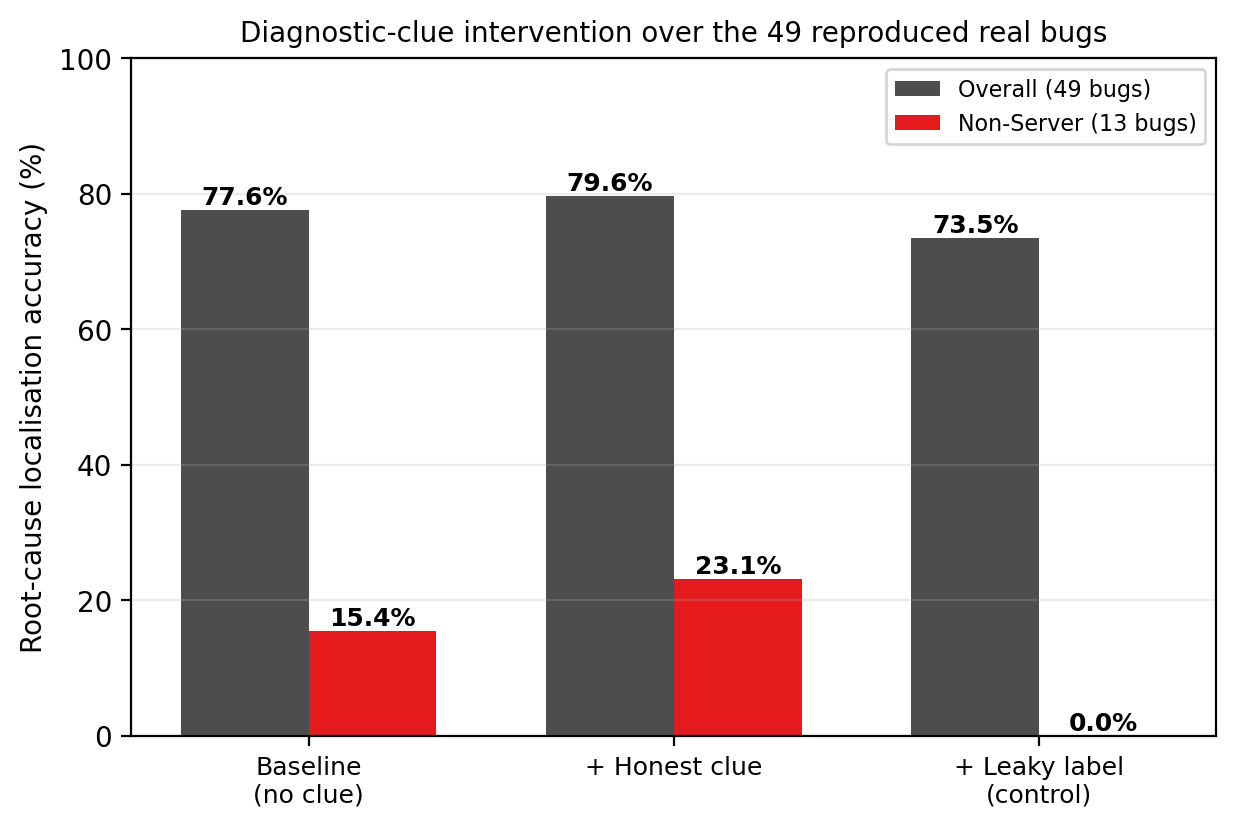
\includegraphics[width=\linewidth]{figs/fig_diag_clues}
  \captionof{figure}{Root-cause localisation accuracy with and without the runnable diagnostic-clue tool over the 49 reproduced real bugs.}
  \label{fig:diag}
\end{minipage}

\begin{table}[!t]
\centering
\caption{How many guesses the surface-text LLM agent needs to localise (reach) the layer where the bug truly originated, over the 49 reproduced real bugs.}
\label{tab:topk}
\scriptsize
\renewcommand{\arraystretch}{1.05}
\setlength{\tabcolsep}{2.5pt}
\begin{tabularx}{\columnwidth}{@{}>{\raggedright\arraybackslash}X >{\centering\arraybackslash}c >{\centering\arraybackslash}c >{\centering\arraybackslash}c@{}}
\toprule
\textbf{Bug subset} & \multicolumn{3}{c}{\textbf{Number of attempts to localise}} \\
\cmidrule(lr){2-4}
& \textbf{1st} & \textbf{2nd} & \textbf{3rd} \\
\midrule
All 49 reproduced bugs & 79.6\% & 87.8\% & 95.9\% \\
13 non-Server bugs (hard) & \textbf{23.1\%} & 53.8\% & 84.6\% \\
\bottomrule
\end{tabularx}
\vspace{0.3em}
\parbox{\columnwidth}{\scriptsize\centering
\textit{Note:} ``Correct on the 1st guess'' means the agent ranks the true root-cause layer first,
i.e.\ it finds the bug on its first attempt; ``2nd guess'' / ``3rd guess'' allow the first two /
three ranked layers, i.e.\ the agent gets up to two / three attempts. The 13 non-Server bugs are
the hard cases, since their faults are not reported at their true origin.}
\end{table}

\subsubsection{Intervention: a runnable diagnostic-clue tool}

We replace the metadata injection with a \emph{runnable diagnostic-clue tool}: a deterministic
module that reads the same SDK text, classifies the run's exposure channel (pushed-to-Server /
silent / caller-exception / single-layer), and emits \emph{directional} guidance --- e.g.\ for a
pushed-to-Server message it advises inspecting the tool-call request (name, argument names,
nesting, types) rather than the tool body, and for a silent result it advises verifying the
returned value's semantics rather than trusting the success flag. Crucially, the tool never
names the origin layer, so it cannot leak the answer; it only packages the observable channel
into actionable direction. Fig.~\ref{fig:diag} shows the effect on the 49 real bugs.

Feeding the agent the tool's guidance raises the \emph{non-Server} localisation accuracy from
\textbf{15.4\%} to \textbf{23.1\%} (+7.7 percentage points), the only place the guidance can help
(the 36 Server-origin bugs are already 100\%). As a negative control we also feed the agent a
bare channel \emph{label} (no guidance); the non-Server accuracy does not improve --- it drops to
\textbf{0.0\%}, slightly below the baseline --- confirming that the benefit comes from the
directional guidance content rather than from any (leakable) channel label. We thus convert the
pain point into a concrete, testable observability improvement without resorting to revealing
ground truth.

\noindent
\begin{tabularx}{\linewidth}{@{}>{\centering\arraybackslash}m{2.2em}!{\vrule width 1pt}>{\arraybackslash}X@{}}
\makecell{\LARGE \faIcon[regular]{lightbulb}} &
\textbf{Finding 5.} A surface-text LLM diagnostic agent achieves 77.6\% overall localisation over the 49 reproduced real bugs, but only 15.4\% on the 13 non-Server-origin bugs (0\% on both Host- and Client-origin faults), misattributing almost all non-Server faults to the Server layer; the non-Server Top-K is only 23.1\% at Top-1 and 84.6\% at Top-3. A runnable diagnostic-clue tool that classifies the exposure channel and points the debugger in the right direction --- without revealing the origin layer --- raises non-Server accuracy to 23.1\% (+7.7 pp), while a leaky channel-label control does not help (0\%). Automated, honest guidance measurably improves localisation of the hard (non-Server) faults.
\end{tabularx}

\textbf{On the earlier metadata intervention.} In an earlier design we attached a structured
\texttt{actual\_fault\_source} field (an enum over the four layers) to every error, which raised
accuracy to $\sim$100\% (ideal) / 93.8\% (realistic). We deliberately \emph{do not} report that
as our result: the field carries the ground-truth origin, so feeding it to the agent effectively
tells it the answer, making the gain circular. We retain it only as an \emph{upper-bound} /
design recommendation, and instead measure the honest improvement of the diagnostic-clue tool,
which never reveals the origin layer. Future work should evaluate the end-to-end accuracy of an
actual origin-tagging generator (e.g.\ a learned classifier or an instrumented SDK wrapper)
against ground truth before claiming a concrete gain.

\subsubsection{Repair experiment: localisation, not fixing, is the bottleneck}

To test whether the diagnostic-clue tool also helps an LLM \emph{repair} a fault (rather than only
localise it), we run a repair experiment. For each fixable case we give the LLM the faulting
source and the SDK output, ask it to produce a corrected runnable script, then re-run it and
verify it no longer errors and returns the expected value. On the earlier
synthetic MCP-Fault-20 subset this showed \textbf{69.6\%} repair success both with and without the
clue --- because with the full faulting source in hand the LLM can read the fault directly and
does not need the clue to localise it, so the clue changes \emph{localisation}
(Fig.~\ref{fig:diag}) but not \emph{repair}. This confirms the paper's central thesis: the
bottleneck in MCP debugging is \emph{localising} the fault (which the clue measurably improves,
from 15.4\% to 23.1\% on the hard non-Server bugs), not \emph{fixing} it once the relevant
code is in hand.

\textbf{Repair on the 49 real bugs is deferred.} The genuine reproduced bugs are
GitHub issues whose ``correct fixed behaviour'' is not auto-verifiable (many need a specific
environment, an authentication server, or a subjective notion of the expected outcome), so an
automated repair-and-verify harness is not directly applicable. We therefore keep the repair
experiment as a complementary result on the auto-verifiable synthetic subset and report this
boundary honestly, rather than fabricating a repair metric for issues we cannot objectively
verify.

\subsubsection{Three technical root causes}

Synthesising the demand-side evidence and the experimental results, we identify three
technical root causes that make MCP fault localisation difficult:
\begin{enumerate}
  \item \textbf{Error reporting carries no root-cause layer metadata.} Errors triggered by
        upstream Host or Client inputs are uniformly surfaced as Server-side tool-execution
        errors, producing manifestation-root-cause mismatch and misleading human debugging.
  \item \textbf{Silent-failure modes exist in default SDK behaviour.} Some erroneous inputs
        are implicitly accepted without raising error flags (11/49 = 22.4\% of the reproduced
        real bugs), making these defects invisible to ordinary monitoring pipelines.
  \item \textbf{Error messages from different layers share similar textual formats.} Without
        structured tags, automated log analysis cannot distinguish the true origin.
\end{enumerate}

Without these controlled experiments, we could only know from interviews that
``fault localisation is hard'' as a subjective complaint. Our experiments over the 49 genuinely
reproduced real bugs further uncover \emph{why} it is hard from an SDK-implementation perspective:
we objectively verify two non-trivial SDK behaviours (manifestation-root-cause mismatch and silent
failure) and show that a runnable diagnostic-clue tool, which packages these channels into
directional guidance without leaking the answer, improves localisation of the hard non-Server
faults (from 15.4\% to 23.1\%).